%% -*- Mode: LaTeX -*-
%%
%% filexfer.tex
%% Created Mon Jun 27 09:39:25 AKDT 2016
%% by Raymond E. Marcil <rmarcil@gci.com>
%% 
%% FileXfer - File Transfer Jobs
%%
%% Links
%% =====
%% Creating Flowcharts with TikZ
%% ShareLaTeX Blog
%% https://www.sharelatex.com/blog/2013/08/29/tikz-series-pt3.html
%%


%%
%%%%%% Preamble.
  %%

%% Specify DVIPS driver used by things like hyperref
\documentclass[12pt,letterpaper,dvips]{article}


%% rcs is the package to display cvs revision info.
%%\usepackage{rcs}
\usepackage{fullpage}
\usepackage{fancyvrb}

%% Decorative lines on header and footer
%% https://www.sharelatex.com/learn/Headers_and_footers
\usepackage{fancyhdr}

\usepackage{graphicx}
\usepackage{figsize}
\usepackage{calc}

%% Tables that span multiple pages
\usepackage{longtable}

%%
%% enumitem – Control layout of itemize, enumerate, description
%% https://www.ctan.org/pkg/enumitem
%%
%% Allows for use of \bgein{itemize}[leftmargin=0pt] 
%% to lists with 0 left margin.
%%
%% Itemize left margin
%% http://tex.stackexchange.com/questions/170525/itemize-left-margin
%% 
\usepackage{enumitem}%     http://ctan.org/pkg/enumitem


%% caption package for use in justifying table or figure captions
\usepackage{caption}

\usepackage{xspace}
\usepackage{booktabs}
\usepackage[first,bottomafter]{draftcopy}
\usepackage[numbib]{tocbibind}

%%
%% Creating Flowcharts with TikZ
%% https://www.sharelatex.com/blog/2013/08/29/tikz-series-pt3.html
%%
\usepackage{tikz}
\usetikzlibrary{shapes.geometric, arrows}

\usepackage{amssymb}              %% AMS Symbols, used for \checkmark
\usepackage{multicol}

%%
%% Extract SVN metadata for use elsewhere.
%% This information has:
%% o the filename
%% o the revision number
%% o the date and time of the last Subversion co command
%% o name of the user who has done the action
%%
%% FIXME: Need to update this for git.
%%
%%\usepackage{svninfo}
%%\svnInfo $Id: filexfer.tex 52 2016-06-27 09:43:54Z marcilr $


%%
%% Including Git Revision Identifiers in LaTeX
%% by Thore Husfeldt
%% https://thorehusfeldt.net/2011/05/13/including-git-revision-identifiers-in-latex/
%% Configure git user name
%%   For individual repo:
%%     $ git config user.name "Bob Jones"
%%
%%   For all repos:
%%     $ git config --global user.name "Bob Jones"
%%
%% Verify user name for repo:
%%   $ git config user.name
%%   Bob Jones
%%
%% Verify user name all repos:
%%   $ git config --global user.name
%%   Bob Jones
%%
%% Changing your username in Git only affects commits that
%% you make after your change.
%%
%% To rewrite your old commits, you can use git filter-branch[1]
%% to change the repository history to use your new username.
%% [1] https://help.github.com/articles/changing-author-info
%%
%%% This file is generated by Makefile.
%%% Do not edit this file!
%%%
\gdef\GITAuthorEmail{marcilr@gmail.com}
\gdef\GITRevision{0.0.1}
	\gdef\GITAbrHash{c35cce8}	\gdef\GITAuthorDate{June 28, 2016}	\gdef\GITAuthorName{Raymond E. Marcil}

%%
%% Hyperref package for embedding URLs for clickable links in PDFs, 
%% also specify PDF attributes here.
%%
%% The pdfborder={0 0 0} is what ellimated the blue box around the url
%% displayed by \href{}{}.
%%
%% The command pdfborder={0 0 1} would display a box with thickness of 1 pt.
%%
%% Hypertext marks in LATEX: a manual for hyperref
%% by Sebastian Rahtz and Heiko Oberdiek - November 2012
%% http://ctan.org/pkg/hyperref 
%% http://mirror.hmc.edu/ctan/macros/latex/contrib/hyperref/doc/manual.html
%%
\usepackage[
colorlinks,
linkcolor=blue,
%%colorlinks=false,
hyperindex=false,
urlcolor=blue,
pdfborder={0 0 0},
pdfauthor={Raymond E. Marcil},
pdftitle={FileXfer File Transfer Jobs},
pdfcreator={ps2pdf},
pdfsubject={FileXfer, file transfer jobs},
pdfkeywords={FileXfer, file transfer jobs}
]{hyperref}


%%
%% Extract RCS metadata for use elsewhere.
%% Jason figured this out, very cool.
%%
%%\RCS $Revision: 1.53 $
%%\RCS $Date: 2006/06/26 21:04:55 $


  %%
%%%%%% Customization.
  %%

% On letter paper with 10pt font the Verbatim environment has 65 columns.
% With 12pt font the environment has 62 columns.  Exceeding this will exceed
% the frame and will look ugly.  YHBW.  HAND.
\RecustomVerbatimEnvironment{Verbatim}{Verbatim}{frame=single}

\renewenvironment{description}
                 {\list{}{\labelwidth 0pt \iteminden-\leftmargin
                          \let\labelsep\hsize
                          \let\makelabel\descriptionlabel}}
                 {\endlist}
\renewcommand*\descriptionlabel[1]{\hspace\labelsep\sffamily\bfseries #1}


  %%
%%%%%% Commands.
  %%

\newcommand{\FIXME}[1]{\textsf{[FIXME: #1]}}
\newcommand{\cmd}[1]{\texttt{#1}}


%% Squeeze space above/below captions
\setlength{\abovecaptionskip}{4pt}   % 0.5cm as an example
\setlength{\belowcaptionskip}{4pt}   % 0.5cm as an example


%% Tex really adds a lot of whitespace to itemized 
%% lists so define a new command itemize* with a 
%% lot less whitespace.  Found this in the British
%% Tex faq.
\newenvironment{itemize*}%
  {\begin{itemize}%
    \setlength{\itemsep}{0pt}%
    \setlength{\parsep}{0pt}}%
  {\end{itemize}}

  
%%
%% Tex really adds a lot of whitespace to itemized 
%% lists so define a new command itemize* with a 
%% lot less whitespace.  Found this in the British
%% Tex faq.
%%
%% Tue Jun 23 13:22:04 AKDT 2015
%% =============================
%% Added [leftmargin=0.0mm] to set the left margin=0
%% This requires use of the enumitem package:
%%   \usepackage{enumitem}%     http://ctan.org/pkg/enumitem
%%
%% Itemize left margin
%% http://tex.stackexchange.com/questions/170525/itemize-left-margin
%%
\newenvironment{itemizenoleft*}%
  {\begin{itemize}[leftmargin=15.0pt]%
    \setlength{\itemsep}{0pt}%
    \setlength{\parsep}{0pt}}%
  {\end{itemize}}
  

%%
%% Tex really adds a lot of whitespace to itemized 
%% lists so define a new command enumerate* with a 
%% lot less whitespace.  Created using itemize*
%% pattern.  
%%
  \newenvironment{enumerate*}%
  {\begin{enumerate}%
    \setlength{\itemsep}{0pt}%
    \setlength{\parsep}{0pt}}%
  {\end{enumerate}}


%%
%% Tex really adds a lot of whitespace to itemized 
%% lists so define a new command enumerate* with a 
%% lot less whitespace.  Created using itemize*
%% pattern.  
%%
%% Tue Jun 23 13:22:04 AKDT 2015
%% =============================
%% Added [leftmargin=0.0mm] to set the left margin=0
%% This requires use of the enumitem package:
%%   \usepackage{enumitem}%     http://ctan.org/pkg/enumitem
%%
%% Itemize left margin
%% http://tex.stackexchange.com/questions/170525/itemize-left-margin
%%
\newenvironment{enumeratenoleft*}%
  {\begin{enumerate}[leftmargin=0.0mm]%
    \setlength{\itemsep}{0pt}%
    \setlength{\parsep}{0pt}}%
  {\end{enumerate}}


%% Squeeze space
\renewcommand\floatpagefraction{.9}
\renewcommand\topfraction{.9}
\renewcommand\bottomfraction{.9}
\renewcommand\textfraction{.1}   
\setcounter{totalnumber}{50}
\setcounter{topnumber}{50}
\setcounter{bottomnumber}{50}

%%
%% The tikzstyle command
%% Now before we start the document we need to define the basic components of
%% a flow chart.  To do this we use the \tikzstyle command.  First let’s
%% define the block we’re going to use for start and stop blocks.  We’ll name
%% it ‘startstop’ using curly brackets immediately following the command, then
%% we add an equals sign before a set of square brackets. In the square
%% brackets we enter all the formatting information. For this block we’ll
%% specify a rectangle with rounded corners.  We’ll give it a minimum width of
%% 3cm and a minimum height of 1cm.  We’ll also ensure the text gets centred
%% and we’ll set both a draw and a fill colour.  In this example we’ve set the
%% fill colour to a colour that is 30% red mixed with 70% white.
%% --sharelatex.com/
%%
\tikzstyle{startstop} = [rectangle, rounded corners, minimum width=3cm,
  minimum height=1cm,text centered, draw=black, fill=red!30]

%%
%% Next we’ll specify an input or output box. This time we want the block to
%% be a parallelogram.  To achieve this we ask for a trapezium and then alter
%% the angles. The rest is very similar.
%% --sharelatex.com/
%%
\tikzstyle{io} = [trapezium, trapezium left angle=70, trapezium right
  angle=110, minimum width=3cm, minimum height=1cm, text centered, draw=black,
  fill=blue!30]

%%
%% Next we’ll add a TikZ style for process blocks using a rectangle and a
%% style for decision blocks using a diamond.
%% --sharelatex.com/
%%
\tikzstyle{process} = [rectangle, minimum width=3cm, minimum height=1cm, text centered, draw=black, fill=orange!30]
\tikzstyle{decision} = [diamond, minimum width=3cm, minimum height=1cm, text
  centered, draw=black, fill=green!30]

%%
%% Finally we’ll define a style for the arrows. For this we set the line
%% thickness to ‘thick’, add an arrow head and specify the stealth arrow head.
%% --sharelatex.com/
%%
\tikzstyle{arrow} = [thick,->,>=stealth]


%%
%% Decorative lines on header and footer
%% Headers and footers
%% https://www.sharelatex.com/learn/Headers_and_footers
%%
%% E for even page
%% O for odd page
%% L for left side
%% C for centered
%% R for right side
%%
\pagestyle{fancy}
\fancyhf{}
%%\fancyhead[CE,RO]{\leftmark}
\fancyhead[RE,LO]{FileXfer}
%% Center like 6 OPERATION
%%\fancyfoot[CE,CO]{\leftmark}
\fancyfoot[LE,RO]{\thepage}

%% FIXME: Need to get initial creation data and current branch here.
\lfoot{Created \GITAuthorDate\hspace{5pt}from \texttt{\jobname.tex}
  (sha-1: \texttt{\GITAbrHash})\\
  by \GITAuthorName \hspace{5pt}\texttt{$<$\GITAuthorEmail$>$}}



  %%
%%%%%% Document.
  %%

\title{FileXfer\\ File Transfer Jobs}

\author{\GITAuthorName\\
        \texttt{$<$\GITAuthorEmail$>$}
%%        \texttt{$<$rmarcil@gci.com$>$}
}

% Display subversion revision and date under author on 1st page.
%%\date{Revision \svnInfoRevision
%%      \hspace{2pt}
%%      (\svnInfoLongDate)}

%%
%% Including Git Revision Identifiers in LaTeX
%% Thore Husfelt
%% https://thorehusfeldt.net/2011/05/13/including-git-revision-identifiers-in-latex/
%%
\date{Revision \GITRevision\hspace{7.5pt}(\GITAuthorDate)}

% Set date to RCS revision date
%%\date{Revision \RCSRevision
%%      \hspace{2pt}
%%      (\RCSDate)}


%%
%% Display SVN (subversion) version data at top right of 1st page,
%% This may be preferable to underneath the author.
%%
%%\rhead{Revision \svnInfoRevision\\
%%\svnInfoLongDate}


%% ===================== Document ======================
%% ===================== Document ======================
%% ===================== Document ======================
\begin{document}

\maketitle


%% ===================== Abstract ======================
%% ===================== Abstract ======================
\begin{abstract}
  \noindent The FileXfer application is a system for automated file transfer
  jobs for copying files.  ``There are 3 applications that make up the usage
  collection framework: \texttt{filexfer}, which does the actual file
  transfers; \texttt{filexfer-jobmonitor}, which is configured
  to monitor various aspects of jobs and create NMS alarms when necessary; and
  \texttt{filexfer-}\\
  \texttt{dataloader}, which bulk-loads file data into database
  tables. There are also housekeeping scripts called
  \texttt{filexfer-filearchive}, which keeps files in the data directory
  pruned and compressed, and \texttt{filexfer-fileunarchive}, which allows
  files to be pulled out of the archive so filexfer jobs can work with them
  again.''\footnote{\href{http://oss-wiki.operations.gci.com/dev/index.php/Usage_Collection\_Framework\_(filexfer)}{Usage Collection Framework (filexfer)}}
\end{abstract}

\vspace{2.0in}

%% Draw DNR logo and address at bottom of page
%%\begin{figure}[h]
%%        \hspace{0.32in}
%%        \SetFigLayout{1}{1}
%%        \begin{minipage}[b]{0.16\figwidth}
%%                \includegraphics[width=\textwidth]{dnr_bwlogo.eps}
%%        \end{minipage}
%%        \hspace{5pt}
%%        \begin{minipage}[b]{\figwidth}
%%                \bf{Alaska Department of Natural Resources}\\
%%                \small{\sf{Division of Support Services\\
%%                Land Records Information Section\\
%%                550 W. 7th Ave. Suite 706\\
%%                Anchorage, Alaska 99501}}
%%        \end{minipage}
%%\end{figure}

\newpage
\tableofcontents

\newpage
\listoffigures
\listoftables


%% =============== List of Abbreviations ===============
%% =============== List of Abbreviations ===============
\newpage
\setcounter{secnumdepth}{0}
\section{List of Definitions and Abbreviations}
\begin{itemize*}
  \item{\begin{bf}MOA\end{bf}} - Municipality of Anchorage

\end{itemize*}


%% ====================== Introduction ===========================
%% ====================== Introduction ===========================
%% ====================== Introduction ===========================
\newpage
\setcounter{secnumdepth}{2}
\section{Introduction}
\fancyhead[LE,RO]{INTRODUCTION}
The FileXfer system...


%% ========================= Design ==============================
%% ========================= Design ==============================
%% ========================= Design ==============================
\newpage
\section{Design}
\fancyhead[LE,RO]{DESIGN}
\FIXME{Need data here...}

%%
%% TikZ flowchart
%% Plenty of notes on creating a TikZ flowchart.
%% Notes on making adjustable size boxes for arbitrary amount of text that I
%% did not use in this exmaple.
%% ShareLaTeX Blog
%% https://www.sharelatex.com/blog/2013/08/29/tikz-series-pt3.html
%% 
\vspace{2cm}
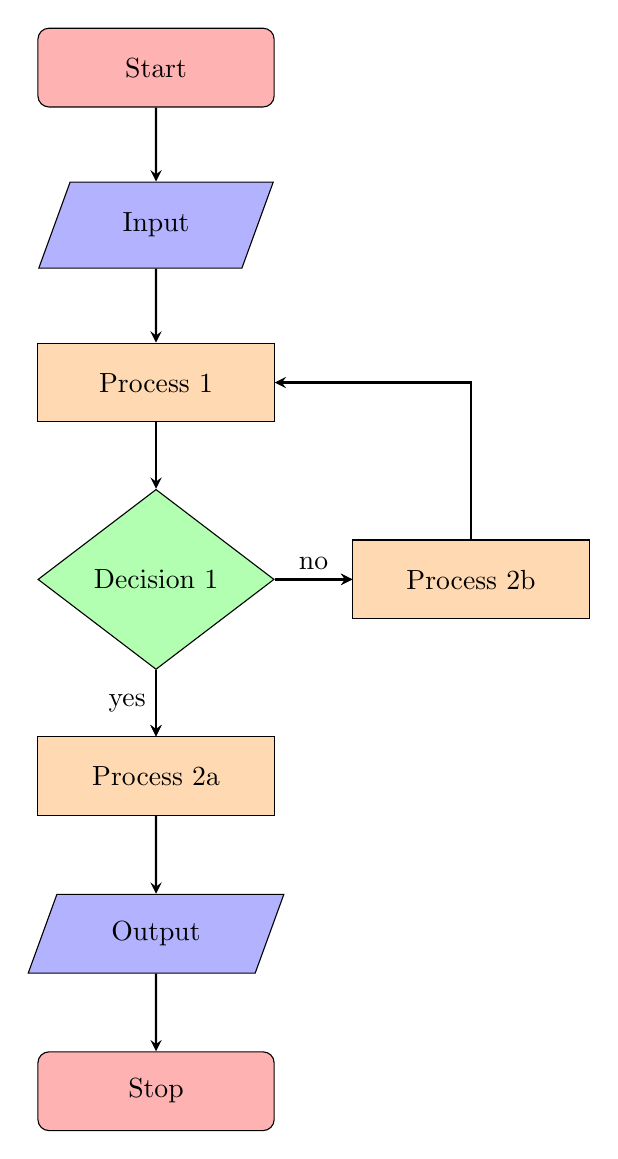
\begin{tikzpicture}[node distance=2cm]

  <TikZ code>

  %% Start block
  \node (start) [startstop] {Start};
  \node (in1) [io, below of=start] {Input};
  \node (pro1) [process, below of=in1] {Process 1};
%%  \node (dec1) [decision, below of=pro1] {Decision 1};
  \node (dec1) [decision, below of=pro1, yshift=-0.5cm] {Decision 1};

  \node (pro2a) [process, below of=dec1, yshift=-0.5cm] {Process 2a};
  \node (pro2b) [process, right of=dec1, xshift=2cm] {Process 2b};
  \node (out1) [io, below of=pro2a] {Output};
  \node (stop) [startstop, below of=out1] {Stop};


  \draw [arrow] (start) -- (in1);
  \draw [arrow] (in1) -- (pro1);
  \draw [arrow] (pro1) -- (dec1);
  \draw [arrow] (dec1) -- (pro2a);
  \draw [arrow] (dec1) -- (pro2b);

  \draw [arrow] (dec1) -- node[anchor=east] {yes} (pro2a);
  \draw [arrow] (dec1) -- node[anchor=south] {no} (pro2b);

  %% Makes diagonal line
%%  \draw [arrow] (pro2b) -- (pro1);

  %% Make the arrow go in a vertical direction before going in a horizontal
  %% direction.
  \draw [arrow] (pro2b) |- (pro1);
  
  \draw [arrow] (pro2a) -- (out1);
  \draw [arrow] (out1) -- (stop);
  
\end{tikzpicture}

\vspace{10pt}
\noindent \FIXME{Customize flowchart FileXfer}


%% ===================== Implementation  =========================
%% ===================== Implementation  =========================
%% ===================== Implementation  =========================
\newpage
\section{Implementation}
\fancyhead[LE,RO]{IMPLEMENTATION}
\FIXME{Need data here...}


%% ========================= Logging ===========================
%% ========================= Logging ===========================
%% ========================= Logging ===========================
\subsection{Logging}


%% ================== Application Logging ======================
%% ================== Application Logging ======================
\subsubsection{Application Logging}
The filexfer applications log to the \texttt{/var/log/filexfer}
directory on \texttt{prod-prov4-cdr1.}\textbackslash\\
\texttt{operations.gci.com}. The parent \texttt{filexfer} jobs
log to \texttt{filexfer-get.log} and
\texttt{filexfer-}\textbackslash\\
\texttt{put.log}.
The \texttt{jobmonitor} and \texttt{dataloader} applications
log to \texttt{jobmonitor.log} and\\
\texttt{dataloader.log}, The \texttt{filexfer} applications
log to the \texttt{/var/log/filexfer} directory on
\texttt{prod-prov4-cdr1.operations.gci.com}. The parent
\texttt{filexfer} jobs
log to \texttt{filexfer-get.}\textbackslash\\
\texttt{log} and \texttt{filexfer-put.log}. The
\texttt{jobmonitor} and \texttt{dataloader} applications log to\\
\texttt{jobmonitor.log} and \texttt{dataloader.log}, respectively. Each file
transfer job is executed as a child process and gets its own log file. The
format is\\
\texttt{filexfer-}$\{$\texttt{neName}$\}$\texttt{-}$\{$\texttt{idJob}$\}$\texttt{-}$\{$\texttt{get,put}$\}$\texttt{.log}.\\
\\
By default, the jobs log at the warn level.  Adjust the level to info to get a
high-level view of the application's state.  Adjust log verbosity by modifying
the appropriate config file in \texttt{/etc/filexfer}.  The changes will take
effect after the next program execution.\\
\\
Errors are also logged to a database table which can be browsed in the
filexfer web interface under the '\texttt{Logs \& Errors}' view.  This view
includes messages logged at \texttt{warn}, \texttt{error}, and \texttt{fatal}
severity.\footnote{\href{http://oss-wiki.operations.gci.com/dev/index.php/Usage_Collection\_Framework\_(filexfer)}{Usage Collection Framework (filexfer)}}


%% ================= File Transfer Logging =====================
%% ================= File Transfer Logging =====================
\subsubsection{File Transfer Logging}
Every file transfer is recorded in a database table. There are
two reasons for this table: first, it tells \texttt{filexfer}
hich files have already been transferred, and second, it
provides an audit trail for SOX compliance. The table is
\texttt{filexfer.logs} on
\texttt{sadc-cdr-mysql1.operations.gci.com}. Use the
\texttt{filexfer.joblogs} view to easily find logs by job name
or network element ID.\\
\\
File transfer logs may also be viewed in the
'\texttt{Logs \& Errors}' page of the web interface.\footnote{\href{http://oss-wiki.operations.gci.com/dev/index.php/Usage_Collection\_Framework\_(filexfer)}{Usage Collection Framework (filexfer)}}


%% =========================== Test ==============================
%% =========================== Test ==============================
\newpage
\section{Test}
\fancyhead[LE,RO]{TEST}
\FIXME{Need data here...}


%% ========================== Issues =============================
%% ========================== Issues  ============================
\newpage
\section{Issues}
\fancyhead[LE,RO]{ISSUES}
\FIXME{Need data here...}


%% ======================== Operation ============================
%% ======================== Operation ============================
%% ======================== Operation ============================
\newpage
\section{Operation}
\fancyhead[LE,RO]{OPERATION}
\FIXME{Need data here...}


%% ===================== Job Scheduling ==========================
%% ===================== Job Scheduling ==========================
\subsection{Job Scheduling}
Jobs are scheduled using a web interface at
\texttt{nms.operations.gci.com/relevance}.  Navigate to the
``FileXfer'' application and click the ``File Transfer Jobs'' link.
Job execution happens on \texttt{prod-prov4-cdr1.operations.gci.com}.
A \texttt{cron} job executes every minute from
\texttt{/etc/cron.d/filexfer} to kick off the various \texttt{filexfer}
scripts.\footnote{\href{http://oss-wiki.operations.gci.com/dev/index.php/Usage\_Collection\_Framework\_(filexfer)}{Usage
    Collection Framework (filexfer)}}


%% =================== Job Timing ================================
%% =================== Job Timing ================================
\subsubsection{Job Timing}
The parent \texttt{filexfer} script is responsible for spawning
child processes for each job. Since a large number of jobs can be
scheduled at any given interval, the parent process limits how
many children can run concurrently.  As long as the limit is
reached and more jobs need to be spawned, the parent process must
stay alive. Since this may take longer than 1 minute, it is
possible for \texttt{filexfer} to miss certain scheduling
intervals.\\
\\
For example, if 500 jobs are scheduled to run at the top of every
hour \texttt{(0 * * * *)} and the maximum child process limit is
50, there is a good chance \texttt{filexfer} will not execute any
jobs scheduled to run at 1 minute past the hour
\texttt{(1 * * * *)}.  The best way to avoid this is to use
\texttt{0}, \texttt{15}, \texttt{30}, or \texttt{45} in the
minute field of the job schedule.  These intervals are always
executed.\footnote{\href{http://oss-wiki.operations.gci.com/dev/index.php/Scheduling\_Usage\_Collection\_Jobs}{Job
    Timing}}




%% ======================= Dataloader ==========================
%% ======================= Dataloader ==========================
\subsection{Dataloader}
Dataloader jobs are configured using the web interface at
\texttt{nms.operations.gci.com/relevance}. Navigate to the
``\texttt{FileXfer}'' application and click the
``\texttt{Data Load Jobs}'' link. These jobs are executed every
minute as long as there are files in the load queue.\footnote{\href{http://oss-wiki.operations.gci.com/dev/index.php/Usage\_Collection\_Framework\_(filexfer)}{Usage Collection Framework (filexfer)}}



%% ======================== Examples =============================
%% ======================== Examples =============================
\newpage
\section{Examples}
\fancyhead[LE,RO]{EXAMPLES}
Series of useful \LaTeX\ markup. Need to break out to 
separate examples.tex file.

\subsection{Escaping $<$ and $>$ Symbols}
To get \$$<$\$ or \$$>$\$ just wrap the symbols in \$ for math mode.

\subsection{Enumerate}
\begin{enumerate}
  \item{DNR} - Alaska State Department of Natural Resources
    \begin{itemize*}
      \item{HI} - Historical Index, not maintained since 1982
      \item{LE} - Land Estate, maintained by SGU
      \item{ME} - Mineral Estate, maintaind by SGU
    \end{itemize*}

  \item{Alaska State Surveys}
    \begin{itemize*}
      \item{ASBLT} - As-Built Survey
      \item{ASCS} - Cadastral Survey
    \end{itemize*}
\end{enumerate}


%% ======================= Comments =======================
%% ======================= Comments =======================
\subsection{Comments}
\begin{center}
\framebox{
\begin{minipage}[t]{0.9\textwidth}
\cmd{COMMENTS} Comment --- \emph{Sean Weems, Spring 2003}\\
We should get the \cmd{COMMENTS} column searchable via the 
landrecords application before we do much anything else -- shouldn't
be too hard.
\end{minipage}
}
\end{center}

\begin{center}
\framebox{
\begin{minipage}[t]{0.9\textwidth}
\emph{Errata: Plats spanning multiple sections}\\
A few anomalies can be observed in the \cmd{AKPLATS}
table. Specifically plats exist that span multiple sections. 
Since the table only has a single column, \cmd{SCODE}, 
that accepts a single section code, SGU (Status
Graphics Unit) has handled this problem by entering multiple 
rows in the table, each with a different section that point to
the same plat or file. Multiple section plats are indicated by  setting 
the \cmd{TCODE} column to the value \cmd{37}, and making an 
appropriate notation like \emph{Section 24-25-26-27} in the 
\cmd{REMARKS} column.\\
\FIXME{Perhaps the \cmd{SCODE} column should accept an array of sections?}

\end{minipage}
}
\end{center}


%% ====================== Footnotes ======================
%% ====================== Footnotes ======================
\clearpage
\newpage
\subsection{Footnotes}
See my
footnote\footnote{\href{http://www.google.com/search?q=latex+footnotes}{Search}
google for footnotes.}
generated with:

\begin{verbatim}
  \footnote{\href{http://www.google.com/search?q=latex+footnotes}
  {Search google for footnotes.}}
\end{verbatim}

\noindent GoogleGuide --- Linking to Search
Results.\footnote{GoogleGuide --- \href{http://www.googleguide.com/linking.html}{Linking to Search Results.}}


%% ====================== Hyperlinks ======================
%% ====================== Hyperlinks ======================
\subsection{Hyperlinks}
Use $\backslash$href\{\} to generate hyperlinks:

\begin{verbatim}
  \href{http://www.google.com}{Google}}
\end{verbatim}

\noindent Yields: \href{http://www.google.com}{Google}


%% ================ Table Examples ================
%% ================ Table Examples ================
\subsection{Table Examples}
\begin{table}[htb]
\begin{tabular}{|p{.25\textwidth}|p{.20\textwidth}|p{.47\textwidth}|}\hline 
Column Name&Type&Description\\ 
\hline
EQS&VARCHAR2(1)&!NULL map shows village selections\\
ITM\_COL&VARCHAR2(1)&USGS ITM column: 1-6\\
ITM\_ROW&VARCHAR2(1)&USGS ITM row: A-E\\
QMQ\_ABBR\_DNR&VARCHAR2(3)&Three character DNR abbreviation for the QMQ\\
RASTER\_FILENAME&VARCHAR2(50)&Physical path to file\\
RASTER\_PATHNAME&VARCHAR2(50)&URL path to PDF of map\\
SCODE&VARCHAR2(2)&Supplement map code: 1,2,3,...\\
COMMENTS&VARCHAR2(256)&Plat comments\\
\hline
\end{tabular}
\caption {\cmd{EASEMENTS\_17B} Table}
\label{table:easements_17b}
\end{table}

%% A simple table example
%% The htb attribute attempts to inline the table or figure
%% where you put it in the document
\begin{table}[htb]
\begin{center}
\begin{tabular*}{\textwidth}{@{}p{.25\textwidth}@{}p{.75\textwidth}}
\hline
\hline\\[-2.5ex]
XML element&Descripton\\
\hline
\hline\\[-1.5ex]   %% Trick to add whitespace after horizontal line
FNUM&US Survey file number\\ 
MERIDIAN&BLM meridian code\\
&\hspace{10pt}12 = Copper River\\
&\hspace{10pt}13 = Fairbanks\\
&\hspace{10pt}28 = Seward\\
&\hspace{10pt}44 = Kateel\\
&\hspace{10pt}45 = Umiat\\
TOWNSHIP&Five character Township code\\
RANGE&Five character Range code\\
PAGE&Survey page number 1,2,3,...\\
FILENAME&Relative path to file in direcory\\[1.5ex]
\hline
\end{tabular*}
\caption {USS XML index elements}
\label{table:uss-index}
\end{center}
\end{table}


%%
%% NOTE: tabular* takes table width argument
%%       Use of 'p' for left aligned column.
%%       Use of 'cp' to center column.
%%       The @{} works to remove an unwanted space.
%%
%% FIXME: Set width of centered columns?
%%
%% Links
%% =====
%% Getting to Grips with Latex - Tables
%% by Andrew Roberts
%% Source for @{\extracolsep{\fill} syntax.
%% http://www.andy-roberts.net/misc/latex/latextutorial4.html
%%
\begin{table}[htb]
\begin{center}
\begin{tabular*}{0.90\textwidth}{@{\extracolsep{\fill}}@{}l@{}c@{}c@{}c}
  \hline
  \hline\\[-2.5ex]
  col 1 & col 2 & col 3 & col 4 \\
  \hline
  \hline\\[-1.5ex]
  item 1 & item 2 & item 3 & item 4 \\
  \hline
  item 1  & item 2  & item 3  & item 4  \\
  \hline
\end{tabular*}
\caption {Demo}
\label{table:demo-index}
\end{center}
\end{table}


%% ================== Installed Daemons ===================
%% ================== Installed Daemons ===================
%% The htb attribute attempts to inline the table or figure
%% where you put it in the document
%%
%% NOTE: tabular* takes table width argument
%%       Use of 'p' for left aligned column.
%%       Use of 'cp' to center column.
%%       The @{} works to remove an unwanted space.
%%
%% FIXME: The ELM adn Elluminate Server columns are not centering.
%%        Center with fixed width in LaTeX?
%%
%% Links
%% =====
%% Getting to Grips with Latex - Tables
%% by Andrew Roberts
%% http://www.andy-roberts.net/misc/latex/latextutorial4.html
%%
%%
%% Configure caption on left using caption package.
%% The key to this working is placing the \captionsetup
%% just before the table or figure for which to manipulate
%% the package.
%%
%% Other potential potential options include:
%%   labelsep=newline
%%   labelfont=bf
%%
%% Links
%% =====
%% Raggedright and caption package
%% http://tex.stackexchange.com/questions/120411/raggedright-and-caption-package
%%
\captionsetup{%
    justification=raggedright,
    singlelinecheck=false
}

\begin{table}[htb]
%%\begin{center}
\begin{tabular*}{.80\textwidth}{@{\extracolsep{\fill}}@{}p{.25\textwidth}@{}c@{}c@{}c@{}c}
\hline
\hline\\[-2.5ex]
Virtual Machine&Apache&ELM&LM&Elluminate Server\\
\hline
\hline\\[-1.5ex]   %% Trick to add whitespace after horizontal line
\cmd{dcs-elive-prod01}&\,&x&x&x\\
\cmd{uaa-elive-dev01}&x&x&x&\\
\cmd{uaa-elive-server01}&\,&\,&\,&x\\[1.5ex]
\cmd{uaa-elive-prod01}&\,&x&x&x\\
\cmd{uaf-elive-prod01}&\,&x&x&x\\
\cmd{uas-elive-prod01}&\,&x&x&x\\
\hline
\end{tabular*}
\caption {Daemons}
\label{table:daemons-index}
%%\end{center}
\end{table}



\begin{table}[htb]
\begin{tabular}{|p{.16\textwidth}|p{.17\textwidth}|p{.62\textwidth}|}\hline 
Column Name&Type&Description\\ 
\hline
MTR&VARCHAR2(9)&Meridian, Township, Range, example: \emph{C026S054E}\\
QMQ&VARCHAR2(3)&Quarter Million Quadrangle code,\\
&&\hspace{10pt}example: \emph{DIL} (Dillingham quadrangle)\\
\hline
\end{tabular}
\caption {\cmd{XREF\_MTR\_QMQ} Table}
\label{table:xref_mtr_qmq}
\end{table}


%% ====================== Verbatim ==========================
%% ====================== Verbatim ==========================
\clearpage
\newpage
\subsection{Verbatim}

``The verbatim environment is a paragraph-making environment that gets
\LaTeX\ to print exactly what you type in. It turns \LaTeX\ into a typewriter
with carriage returns and blanks having the same effect that they would
on a typewriter.''\footnotemark

\begin{verbatim}
\begin{verbatim}
    text
\end{verbatim\}
\end{verbatim}


%% ========= Figure formatting with verbatim ===============
%% ========= Figure formatting with verbatim ===============
\noindent\begin{bf}Figure formatting with verbatim\end{bf}\\
%%
%% Making Figures in LaTeX
%% The [htb] part above advises LaTeX to put the figure "here"
%% or at the "top" or " bottom" of the page, with that order of preference.
%% http://www.sci.utah.edu/~macleod/latex/latex-figures.html
%%
\noindent The following figure leverages verbatim for proper formatting:
\vspace{-5mm}
\begin{center}
\begin{figure}[htb]
\begin{quote}
\small
\begin{Verbatim}[frame=none]
gis/raster/
  dnr/
    map_library/
    plats/
      SP/YYYYMMDD/*.pdf               # indexed
      HI/YYYYMMDD/*.pdf               # Indexed
      ASLS/YYYYMMDD/*.pdf             # Indexed
    recorded-plats/
      YYYYMMDD/*.pdf
  blm/
    easements_17b/YYYYMMDD/*.pdf      # indexed
    mtp/YYYYMMDD/*.pdf                # non-indexed
    usrs/YYYYMMDD/*.pdf               # indexed
    usrs-notes/YYYYMMDD/*.pdf         # indexed
    uss/YYYYMMDD/*.pdf                # indexed
    uss-notes/YYYYMMDD/*.pdf          # indexed
    usms/YYYYMMDD/*.pdf               # indexed
    usms-notes/YYYYMMDD/*.pdf         # indexed
  usgs/
    drg/
      collared/ 
        250K/
        63K/
        25K/
        24/
      decollared/
      tools/
      missing\_data/
    dem/
    doq/
    topo/
\end{Verbatim}
\normalsize
\end{quote}
\caption{File and Directory Structure}
\label{fig:dirlayout}
\end{figure}
\end{center}



%% ======================== Appendix =============================
%% ======================== Appendix =============================
%% ======================== Appendix =============================
%%
%% This will add a standard non-numbered Appendix to the document.
%% The next section Appendix chnages secnumdepth such that the Appendix
%% is not numbered but still displayed in the table of contents (TOC).
%%
%% Adding unnumbered sections to TOC
%% http://tex.stackexchange.com/questions/11668/adding-unnumbered-sections-to-toc
%% 
%% \section*{Appendix}
%% Need content here.
%%
\setcounter{secnumdepth}{0}
\section{Appendix}
\fancyhead[LE,RO]{APPENDIX}


%% ========================= Source ==============================
%% ========================= Source ==============================
\subsection{Source}
Code from
\texttt{prod-prov4-cdr1}\footnote{\texttt{prod-prov4-cdr1.operations.gci.com}
  (\texttt{192.168.161.47}, NATed IP: \texttt{66.223.199.228}), data including
  CDRs and such under \texttt{/data/usage/} ---
  Network Services, OSS.}

\vspace{20pt}
\noindent\FIXME{Need data here}

\begin{longtable}[l]{ll}
%%    \label{FileXfer directories and files on prod-prov4-cdr1}
    \multicolumn{2}{c}%
    {{\bfseries \tablename\ \thetable{} -- FileXfer directories and files on \texttt{prod-prov4-cdr1}}} \\
    \hline
    \multicolumn{1}{|l|}{\textbf{Directory}} &
    \multicolumn{1}{l|}{\textbf{File(s)}}\\
    \hline
\endfirsthead

\multicolumn{2}{c}%
{{\bfseries \tablename\ \thetable{} -- continued from previous page}} \\
\hline
\multicolumn{1}{|l|}{\textbf{Directory}} &
\multicolumn{1}{l|}{\textbf{File(s)}} \\ \hline 
\endhead

\hline \multicolumn{2}{|r|}{{Continued on next page}} \\ \hline
\endfoot

%% This was double horizontal lines at end of table.
%%\hline \hline
\endlastfoot

    \texttt{/etc/filexfer/}&\texttt{*.conf}\\
    \texttt{/usr/bin/}&\texttt{filexfer-dataloader}\\
    &\texttt{\textbf{filexfer-dataloader.plx}}\\
    &\texttt{filexfer-dataloader.plx.mbak}\\
    &\texttt{filexfer-epg-dataloader.plx}\\
    &\texttt{filexfer-filearchive}\\
    &\texttt{filexfer-filearchive.sh}\\
    &\texttt{filexfer-fileunarchive}\\
    &\texttt{filexfer-fileunarchive.sh}\\
    &\texttt{filexfer-jobmonitor}\\
    &\texttt{\textbf{filexfer-jobmonitor.plx}}\\
    &\texttt{\textbf{filexfer.plx}}\\
    \texttt{/usr/lib/filexfer}/&\texttt{*.gz, *.sh, *.plx}\\
    &\texttt{ExtractCarrierTurboZoneUsage*}\\
    \texttt{/usr/share/filexfer}/&\texttt{filexfer.changelog-*.xml}\\
    &\texttt{filexfer.changelog-master.xml}\\
    &\texttt{liquibase.sh}\\
    &\texttt{.gnupg/pubring.gpg}\\
    &\texttt{.gnupg/random\_seed}\\
    \texttt{/var/cache/yum/build/packages/}&\texttt{filexfer-0.52-1.el5.centos.noarch.rpm}\\
    \texttt{/var/lib/filexfer/}
    &\texttt{dataloader.kch}\\
    &\texttt{dataloader\_temp.kch}\\
    &\texttt{filexfer-aaa01-13-get.kch}\\
    &\texttt{...}\\
    &\texttt{filexfer-wps01-706-get.kch}\\
    &\texttt{filexfer.kch}\\
    &\texttt{jobmonitor-mailstat.kch}\\
    &\texttt{jobmonitor.kch}\\
    \texttt{/var/log/filexfer}&\texttt{*.log}\\
    &\texttt{ExtractCarrierTurboZoneUsage\_ACS.log}\\
    &\texttt{archive}\\
    &\texttt{convert-wps-om-counters-report-part2.log}\\
    &\texttt{convert-wps-om-counters-report.log}\\
    &\texttt{\textbf{dataloader.log}}\\
    &\texttt{dataloader\_temp.log}\\
    &\texttt{dataloadinsert.log}\\
    &\texttt{datarecovery.log}\\
    &\texttt{epg-dataloader.log}\\
    &\texttt{ericsson-oss-rl-reports-preprocess.log}\\
    &\texttt{ericsson-oss-sts-reports-preprocess.log}\\
    &\texttt{filearchive.log}\\
    &\texttt{filexfer-aaa01-13-get.log}\\
    &\texttt{filexfer-aaa01-14-put.log}\\
    &\texttt{...}\\
    &\texttt{/var/log/filexfer/filexfer-wps01-706-get.log}\\
    \hline \hline
\end{longtable}


%% ========================== Links ==============================
%% ========================== Links ==============================
\subsection{Links}
%% ============= LaTeX - Wikibooks ===============
A Guide to \LaTeX\\\
\href{http://www.astro.rug.nl/~kuijken/latex.html}
{http://www.astro.rug.nl/~kuijken/latex.html}
\\
\\
\LaTeX\ - From Wikibooks,the open-content textbooks collection\\
\href{http://en.wikibooks.org/wiki/LaTeX}{http://en.wikibooks.org/wiki/LaTeX}
\\
\\
\LaTeX\ Notes\\
\href{http://luke.breuer.com/time/item/LaTeX\_Notes/180.aspx}{http://luke.breuer.com/time/item/LaTeX\_Notes/180.aspx}

\end{document}

%% Local Variables:
%% fill-column: 78
%% mode: auto-fill
%% compile-command: "make"
%% End:
